\chapter{软件相关技术概述}

本章将对农业果实称重云端软件所使用的相关技术进行概述,包括 Spring 技术栈、YOLO 目标检测算法、基于 GTID 的主从复制技术、MQTT 消息传输协议以及 EMQX 网关框架这五种技术。

\section{Spring 技术栈}\label{sec:spring}

农业果实称重云端软件使用 Spring 技术栈来构建整个后台服务,技术栈包括了核心的 Spring 框架,以及两个重要的基于 Spring 的框架:Spring Security 和 Spring Boot。

\begin{figure}[H]
    \centering
    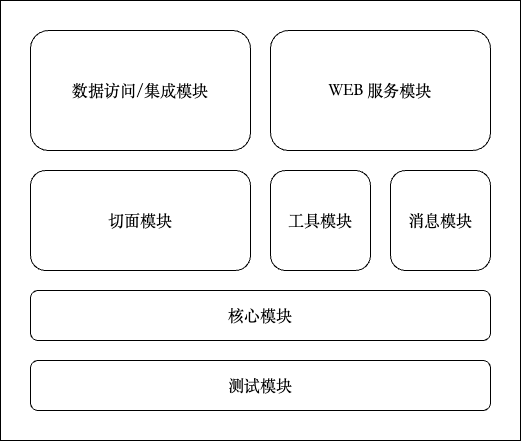
\includegraphics[width=0.8\linewidth]{../design/out/Spring.png}
    \caption{Spring 七大模块}
    \label{fig:Spring}
\end{figure}

Spring 框架主要提供了七大模块的功能,分别是数据访问/集成模块、WEB服务模块、切面模块、工具模块、消息模块、核心模块以及测试模块,如图\ref{fig:Spring}所示;Spring Security 框架为软件提供了可靠的安全保障,确保了外部请求的安全性;Spring Boot 框架提供了简化应用开发和配置的能力,帮助快速构建和部署云端应用。

Spring 框架中的核心模块提供了 IOC(控制反转)和 DI (依赖注入)这两大功能;切面模块提供了 AOP (面向切面编程)支持;数据访问/集成模块主要提供了对象关系映射、事务、数据库连接、Java 消息服务以及对象 XML 映射这五个功能;Web 服务模块为应用提供了编解码、过滤器、跨域、WebFlux(响应式 Web 编程)、WebMVC(模型-视图-控制器模式)等功能;工具模块则为应用提供了服务监控、日志记录等扩展功能;消息模块提供了丰富易用的消息队列集成;测试模块则为应用提供了强大的单元测试支持\cite{Spring-框架概述}。

\begin{figure}[H]
    \centering
    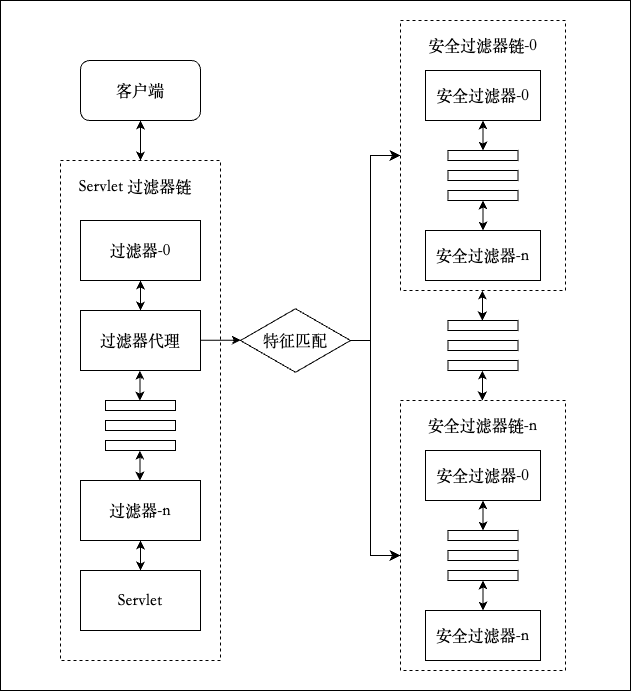
\includegraphics[width=0.8\linewidth]{../design/out/Spring-Security.png}
    \caption{Spring Security 请求过滤流程}
    \label{fig:Spring-Security}
\end{figure}

Spring Security 是 Spring 框架的安全扩展,专门用于解决应用的安全需求,通过与 Spring 的各个模块的集成,提供了一种高度灵活且易于配置的安全方案。Spring Security 提供了强大而灵活的安全过滤器,用于对用户进行认证和授权,其请求过滤流程如图\ref{fig:Spring-Security}所示,图中左侧的请求链是 Servlet 定义的过滤器链,右侧的请求链是 Spring Security 定义的安全过滤器链。客户端发起一个 HTTP 请求,请求首先到达 Servlet 过滤器链,其中过滤器0至过滤器n是普通的 Servlet 过滤器,通常用于执行非安全相关的任务如日志记录、性能监控、数据压缩等。Spring Security 所提供的过滤器代理委托者将会在 Servlet 过滤器链中拦截到该请求,将请求委托给过滤器代理,过滤器代理将根据请求的特征选择一个匹配的安全过滤器链,依次对请求进行处理(例如身份验证、授权等)。如果所有过滤器都允许该请求通过,则请求最终到达 Servlet 进行业务逻辑处理。Servlet 生成响应,响应同样会经过滤器链返回给客户端。如果在安全过滤器链的任何阶段,请求未能通过安全检查(例如身份验证失败或未授权),则会根据配置返回相应的错误响应\cite{Spring-Security-架构设计}。

Spring Boot 是建立在 Spring 框架之上的一款开发工具,旨在简化应用程序的构建、配置和部署流程。Spring Boot 提供了自动化配置和内嵌服务器支持,大大减少了 Spring 应用所需的配置工作。它通过提供预设的默认配置和自动化配置机制,使开发者能够专注于业务逻辑开发,免去了处理繁琐底层配置的负担\cite{Spring-Boot-概述}。

综上所述,农业果实称重云端软件采用的 Spring 技术栈通过 Spring、Spring Security 和 Spring Boot 的紧密结合,提供了强大的功能支持和灵活的扩展性。

\section{YOLO 目标检测算法}\label{sec:yolo}

YOLO(You Only Look Once)是一种高效的目标检测算法,因其速度快、精度高的特点,在计算机视觉领域被广泛应用于实时目标检测任务\cite{Lin2019}。在农业果实称重云端软件中,应用 YOLO 来训练果实图像检测模型,实现果实种类的检测与识别。YOLO 的检测原理可以从图像划分、目标预测、损失函数和后处理四个方面阐述。

(1)图像划分:YOLO 将输入的图像划分为多个网格单元,各单元分别预测中心点落在单元内的目标。这种划分方式使得算法能够快速定位目标的大致位置,提高检测效率\cite{Liu2023-yolov8}。

(2)目标预测:对于每个网格单元,YOLO 预测多个边界框和对应的类别概率。边界框包含了目标的位置信息,通常用四个坐标值表示。类别概率表示该边界框内目标属于各个类别的可能性\cite{Liu2023-yolov8}。

(3)损失函数:YOLO 采用一种多任务损失函数,综合优化模型参数,涵盖边界框回归、类别分类和物体置信度等多个目标检测任务\cite{Liu2023-yolov8}。损失函数通常由分类损失和回归损失组成。分类损失用于衡量模型对目标类别的预测准确性,回归损失用于衡量模型对目标边界框的预测准确性。

(4)后处理:在预测完成后,YOLO 通常采用一些后处理方法,如非极大值抑制(Non-Maximum Suppression,NMS)或软非极大值抑制(Soft-NMS, Soft Non-Maximum Suppression)\cite{Lin2019},来去除重复的检测结果,提高检测的准确性。

\section{基于 GTID 的主从复制技术}\label{sec:gtid}

在农业果实称重云端软件中,使用了 MySQL 数据库来存储大量数据,数据存储分为主库存储和从库存储。主库完成数据的读写,而从库只进行数据的读取。为实现主从库数据的一致性,采用了基于全局事务标识符 (GTID, Global Transaction Identifier) 的主从复制技术来完成数据同步操作。GTID 由服务器全局唯一标识符(UUID, Universally Unique Identifier) 和事务编号组成,是一个在 MySQL 数据库中用于唯一标识一个事务的标识符。

\begin{figure}[H]
    \centering
    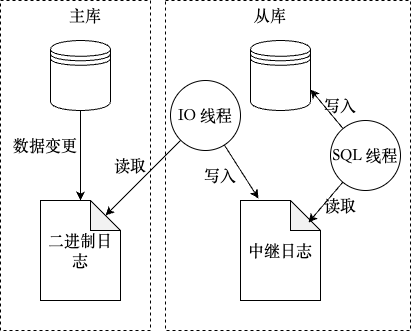
\includegraphics[width=0.8\linewidth]{../design/out/GTID-Replication.png}
    \caption{主从复制流程}
    \label{fig:GTID-Replication}
\end{figure}

MySQL 所实现的主从复制技术性能优越,其内置的复制流量压缩选项可将总网络流量最多减少 20\%\cite{shehzad2020networkfootprintreplicationpopular}。其主从复制的流程如图\ref{fig:GTID-Replication}所示,左侧为主库,右侧为从库,具体执行解释如下:

1、主库在执行事务时,会为每个事务分配一个唯一的 GTID,并将该 GTID 记录在二进制日志中。

2、从库连接到主库后,读取主库二进制日志并将其写入本地的中继日志。根据其中的 GTID 来判断哪些事务已经执行过,哪些事务需要执行。如果一个事务的 GTID 不在从库的已执行事务集合中,从库就会执行该事务。

3、从库在执行事务时,也会为每个事务分配一个 GTID,并将其记录在自己的二进制日志中。这样,从库也可以作为其他从库的主库,实现级联复制\cite{MySQL-Liu2022}。

\section{MQTT 消息传输协议}\label{sec:mqtt}

MQTT(Message Queuing Telemetry Transport)即消息队列遥测传输协议,是一种轻量的消息传输协议。本软件采用 MQTT 作为称重消息的发布/订阅的通信协议,使用 EMQX(Erlang MQTT Broker) 作为 MQTT 消息发布服务器。EMQX 是开源软件,不仅性能表现优越,而且支持多种版本的 MQTT 协议\cite{dizdarevic2023engineeringexperimentallybenchmarkingopen}。在软件中,发送 MQTT 消息上传称重信息具有以下优势:

(1)低带宽和低功耗:MQTT 协议采用轻量消息格式与高效发布/订阅机制,适用于带宽受限、能耗敏感的物联网环境。对于电子秤等设备,可在网络资源有限或移动场景下稳定传输称重数据,降低通信负载与能耗\cite{Jia2015}。

(2)实时性和可靠性:MQTT 协议支持通过 QoS(Quality of Service,服务质量)来控制传输质量。可以根据不同的应用需求,选择不同的消息传输质量级别。在 MQTT 协议中,QoS 有三种级别\cite{Jia2015},分别是 QoS0、QoS1 和 QoS2,分别代表消息最多传送一次、消息至少传送一次和消息只传送一次。软件要求称重消息有且仅被消费一次,则应该选择 QoS2 级别,确保消息的可靠传输。

% QoS0 – “最多一次”:消息最多传送一次,不保证消息到达目标。适用于实时性要求非常高,但对消息丢失容忍的场景;

% QoS1 – “至少一次”:保证消息至少传送一次,但可能会重复。适用于需要消息可靠到达,但不介意重复接收的情况;

% QoS2 – “只有一次”:确保每条消息只会传送一次,且无重复。适用于对消息的唯一性和可靠性有较高要求的场景。

(3)易于扩展和集成:MQTT 协议可以轻松地与其他物联网协议进行集成,如 CoAP、WebSocket、HTTP 等。MQTT 协议的发布/订阅模式支持大规模的设备连接和数据传输,适用于构建物联网应用平台。例如,在智慧农业大棚测控系统中,采用 MQTT 协议将大棚内的测控系统和物联网云平台进行结合,通过移动终端访问云服务器数据库,实现了对农业大棚的实时监测和控制\cite{Liang2020}。

\section{EMQX 网关框架}\label{sec:emqx}

在农业果实称重云端软件中,为支持更多电子秤协议的接入,采用了 EMQX 网关框架,将多种不同物联网应用层协议在网关处转换为 MQTT 协议,使用 MQTT 协议继续进行后续的通信。框架提供了统一的用户层接口和会话/连接管理。各个协议的客户端有独立的认证器和监控器\cite{EMQX-Gateway}。其整体的架构如图\ref{fig:EMQX-Gateway}所示,左侧展现了 EMQX 网关的分层架构,右侧展现的是 MQTT 发布/订阅核心组成。在 EMQX 网关分层架构中,左下角显示了包括 MQTT-SN、Stomp、CoAP 等在内的多种协议,这些协议有着独立的认证器来完成认证和监控器来进行客户端级别的指标统计功能。

\begin{figure}[H]
    \centering
    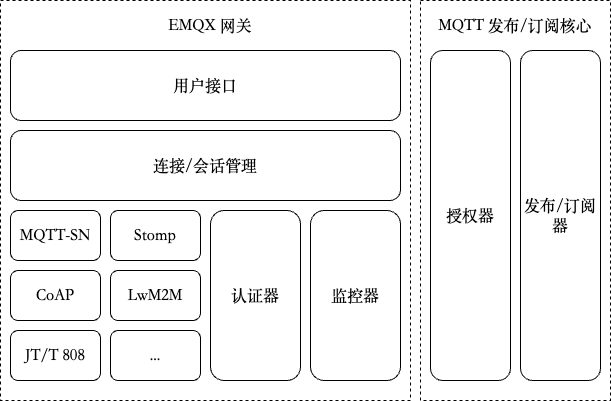
\includegraphics[width=0.8\linewidth]{../design/out/EMQX-Gateway.png}
    \caption{EMQX 网关框架架构}
    \label{fig:EMQX-Gateway}
\end{figure}

不同协议的消息进入网关后,首先完成认证,认证通过后将会进行消息模型的转换,将消息内容转换成为 MQTT 格式的内容,并以 MQTT 协议进行后续的通信。通过 MQTT 授权器完成授权功能,最后执行发布和订阅动作。

\section{本章小结}

本章对软件所使用的相关技术进行了概述,包括 Spring 技术栈、YOLO 目标检测算法、基于 GTID 的主从复制技术、MQTT 消息传输协议以及 EMQX 网关框架这五种技术。这些技术的结合为软件的高效运行和数据处理提供了有力保障。
